% ====================
% Plan for Completion
% ====================
\chapter{Plan for Completion}

% ====================
% Research Contributions and Future Works
% ====================
\section{Research Contributions}
\label{sec:contribution}
In my DPhil research, I am developing interpretable deep learning methods to quantify fetal brain development from 3D ultrasound. In current clinical practice, fetal brain development is monitored with routine ultrasound examinations. During these examinations, brain development is assessed using a number of in-plane measurements, such as the trans-cerebellar diameter. However, the information obtained from these in-plane measurements is limited, and new insights that can potentially be discovered with an in-depth analysis of 3D ultrasound scans are therefore mostly unexplored. For this reason, in my doctoral research, I am developing novel methods to obtain improved insight in fetal brain development, such as automated subcortical segmentation (Contribution 1) and brain age prediction of specific cortical regions (Contribution 2). Furthermore, I aim to develop methods that are \textit{interpretable}, so that these methods can eventually be translated to clinical care.

In the remainder of this section, I will summarize each of the three contributions that my DPhil thesis will contain.  


\begin{enumerate}[wide,label=\Roman*, labelindent=0pt]

\item \textbf{Subcortical Segmentation of the Fetal Brain in 3D Ultrasound using Deep Learning}

\noindent During routine pregnancy monitoring, several subcortical structures are measured to assess the growth and health of the fetal brain, illustrating the importance of these structures. To study the development of these structures in more detail, segmentations of the individual structures are required. However, manual delineation of several structures in 3D ultrasound volumes is extremely time-consuming and challenging. For this reason, in my first contribution I have studied the automated segmentation of several subcortical structures in 3D ultrasound volumes using a convolutional neural network (CNN). A schematic overview of the pipeline of this method is shown in Fig. \ref{fig:contr1}. As obtaining manual annotations for training is costly, I specifically studied training CNN's for this task in a low-data regime. I compared using a small number of individually annotated volumes versus using many weakly labelled volumes obtained from atlas-based segmentations. Furthermore, I also applied the trained models to a cohort of healthy fetuses, obtaining US-specific growth curves for subcortical growth during the second trimester of gestation. 

The work for this contribution has been published as a journal publication in NeuroImage:

\noindent \textbf{L.S. Hesse}, M. Aliasi, F. Moser, the INTERGROWHT-21st Consortium, M.C. Haak, W. Xie, M. Jenkinson, and A.I. Namburete : Subcortical Segmentation of the Fetal Brain in 3D Ultrasound using Deep Learning.

\begin{figure}
	\centering
	\includegraphics[width=  \textwidth]{Figures/Methods3D_Figure.png}
	\caption{Schematic Overview of Contribution 1: Segmentation of subcortical structures (Choroid Plexus (orange), Lateral Posterior Ventricle Horn (yellow), Cerebellum (pink), and Cavum Septum Pellucidum et Vergae (green)) in 3D ultrasound under a low-data regime.}
\label{fig:contr1}
\end{figure}


\item \textbf{Assessment of Cortical Development using Fissure Based Age Prediction}

\noindent \textit{This chapter will contain collaborative work between me and Madeleine Wyburd.}

\noindent The folding of the cortical plate has been found to be temporally consistent in healthy fetuses. For this reason, the degree of folding can be used to assess fetal brain development. However, while manual grading charts to quantify this relationship exist, these tend to be extremely user-dependent therefore not suitable for large scale implementation in clinic. For this reason, we developed a method that assesses the development of several individual fissures by predicting the gestational age of the respective region. As in a healthy cohort gestational age and fissure appearance is assumed to be well correlated, we trained our model with scans from a group of healthy fetuses using the gestational age as ground-truth. Our model can subsequently be applied to diseased cohorts, in which the difference between predicted and true gestational age for each fissure can give an indication of local advanced or delayed cortical folding. 

A schematic overview of this method is shown in Fig. \ref{fig:contr2}. In order to assess individual fissure development, we first extracted a bounding box around each of the fissures of interest, and subsequently predicted the gestational age of these regions using separate CNN's for each fissure. Going forward, we aim to merge the separate networks into a single architecture that predicts an age for each of the fissures directly from a whole brain ultrasound scan (thus, removing step 1 from Fig. \ref{fig:contr2}). Furthermore, we plan to incorporate attention in the network to make it more interpretable. 

Part of this work has been presented as an oral presentation at ISUOG 2021 (International Society of Ultrasound in Obstetrics and Gynecology), as well as published as a workshop paper in PIPPI 2021 (MICCAI affiliated workshop on Perinatal Imaging, Placental and Preterm Image Analysis):

\noindent \textbf{L.S. Hesse\footnote[1]{Indicates equal contribution}}, M.K. Wyburd\footnotemark[1], M. Aliasi, M. Jenkinson, A.T. Papageorghiou, M.C. Haak, and Namburete A.I.:  "Assessment of Regional Cortical Development Through Fissure Based Gestational Age Estimation in 3D Fetal Ultrasound." \textit{Uncertainty for Safe Utilization of Machine Learning in Medical Imaging, and Perinatal Imaging, Placental and Preterm Image Analysis.} Springer, Cham, 2021. 242-252.


\begin{figure}[t]
	\centering
	\includegraphics[width= 0.9 \textwidth]{Figures/Cortical Age Project.png}
	\caption{Schematic Overview of Contribution 2: Cortical Age Prediction of individual fissures consisting of 1) Bounding box selection around the fissures of interest, and 2) gestational age prediction for each fissure separately.}
\label{fig:contr2}
\end{figure}


% ====================
% Figure -  Seg pipeline
% ====================
%\begin{figure*}
%\includegraphics[width=\textwidth]{fig/Figure1.png}
%\centering
%\includegraphics[width=\textwidth]{Figures/pipeline_corticalaging.pdf}
%\vspace{-15pt}
%\caption{Pipeline  (Contribution \#2).
%} 
%\label{seg}
%\vspace{-16pt}
%\end{figure*}



\item \textbf{Interpretable Age Prediction using Similarity Based Examples} 

\noindent As detailed in Contribution 2, fetal brain age prediction can provide valuable information about fetal brain development. However, in order to implement these methods in clinical care, it is essential that problems in the decision-making process of the model can be identified before deployment. Conventional CNN's are typically non-interpretable, making it challenging to identify problems in the reasoning process of the model. For this reason, in my my third contribution I will study age prediction using an inherently interpretable CNN that can explain its reasoning process by providing similar examples from the training dataset. 

As earlier work on such interpretable CNN's has only focussed on classification tasks, I have first developed an interpretable CNN for regression using a large, publicly available dataset on diabetic retinopathy grading. This work has been submitted as a conference paper to MICCAI 2022 and was included in Chapter \ref{chapter1}. For my thesis, I will extend these methods and apply them to (a) adult brain aging in MRI, and (b) fetal brain development in ultrasound.


\end{enumerate}


\subsection*{Clinical Application}
To demonstrate my developed methods on a clinical dataset, I will also apply the models to a clinical dataset containing fetuses with congenital heart disease (CHD). Children with CHD show a delayed cognitive development in childhood, however, it is not yet known what the developmental origin of this delay is. For this reason, studying brain development of fetuses with CHD is of clinical interest, as it can potentially provide new insights in the differences in brain development between healthy fetuses and fetuses with CHD. This study is a collaboration with the Leiden University Medical Center (LUMC), for which we are doing the data analysis. A first clinical paper applying my subcortical segmentation method (Contribution \RomanNumeralCaps{1}) to extract volumetric development is currently in writing, and we also plan a second paper applying the cortical aging network (Contribution \RomanNumeralCaps{2}). 


% ====================
% Thesis Chapters Organisation
% ====================
\section{Proposed Thesis Outline}

The proposed outline of my thesis is summarized below. The percentages shown after each (sub-)section indicate how much of the task is completed at the confirmation submission time.

\begin{enumerate}
\item Introduction [20\%]

\item Literature Review [40\%]

\item \textbf{Contribution \RomanNumeralCaps{1}}: Subcortical Structure Segmentation of the Fetal Brain from 3D ultrasound 
\begin{enumerate}
  \item Technical Contribution: Subcortical Segmentation using deep learning in a low-date regime [95\%]
  \item Clinical application: subcortical brain development in CHD fetuses [80\%]
\end{enumerate}

\item \textbf{Contribution \RomanNumeralCaps{2}}: Assessment of Cortical Development using Fissure Based Age Prediction
\begin{enumerate}
  \item Technical Contribution: Age prediction of individual fissures from 3D fetal brain ultrasound [50\%]
  \item Clinical application: fissure development in CHD fetuses  [30\%]
\end{enumerate}

\item \textbf{Contribution \RomanNumeralCaps{3}}: Interpretable Deep Learning for Regression
\begin{enumerate}
  \item Proof-of-concept using Diabetic Retinopathy Grading [100\%]
  \item Use Case 1: Adult rain aging in MRI [0\%]
  \item Use Case 2: Fetal brain development in US [0\%]
\end{enumerate}



\item Conclusion [0\%]

\end{enumerate}



\hfill
% ====================
% Timetable
% ====================
\section{Proposed Timetable}
\label{sec:timetable}
An overview of the proposed timeline for completion of the DPhil thesis is outlined in a Gantt Chart in Fig. \ref{fig:gantt}. Between June and September 2022 I will be temporarily suspending my DPhil to do a 3-month research internship at Microsoft Research Cambridge.

\begin{figure}[h]
  \begin{center}
  
  \begin{ganttchart}[Mile1/.style={milestone/.append style={fill=red}},
    y unit title=0.6cm,
  y unit chart= 0.6 cm,
  x unit = 0.6cm,
  vgrid,hgrid, 
  title label anchor/.style={below=-1.6ex},
  title left shift=.05,
  title right shift=-.05,
  milestone left shift = 0.75,
  milestone right shift = 0.25,
  title height=1,
  progress label text={},
  bar height=0.7,
  group right shift=0,
  group top shift=.6,
  group height=.3]{1}{15}
  %labels
  \gantttitle{2022}{9} 
  \gantttitle{2022}{6} \\
  \gantttitle{4}{1}
  \gantttitle{5}{1}
  \gantttitle{6}{1} 
  \gantttitle{7}{1} 
  \gantttitle{8}{1} 
  \gantttitle{9}{1} 
  \gantttitle{10}{1}
  \gantttitle{11}{1} 
  \gantttitle{12}{1}
  \gantttitle{1}{1}
  \gantttitle{2}{1}
  \gantttitle{3}{1}
  \gantttitle{4}{1}
  \gantttitle{5}{1}
  \gantttitle{6}{1}\\
  %tasks


  \ganttgroup{\RomanNumeralCaps{1} Subcortical Segmentation}{1}{2} \\
  \ganttmilestone[Mile1]{Finish Clinical Paper}{1}{2} \\

  \ganttgroup{Microsoft Research Internship}{3}{5}\\

  \ganttgroup{\RomanNumeralCaps{2} Cortical Age Prediction}{1}{8} \\
  \ganttbar{Improve Interpretability}{1}{2} \\
  \ganttmilestone[Mile1]{Finish Technical Paper draft}{2}{3}\\
  \ganttbar{Apply to LUMC dataset}{2}{2} \\

  
  \ganttbar{Finalize Technical Paper}{6}{8} \\
  \ganttmilestone[Mile1]{Submit Technical Paper}{8}{9}\\
  \ganttbar{Finalize Clinical Paper}{6}{8} \\
  \ganttmilestone[Mile1]{Submit Clinical Paper}{8}{9}\\



  \ganttgroup{\RomanNumeralCaps{3} Interpretable Regression}{1}{12} \\
 
  \ganttbar{Finish Methods DR Grading}{1}{1} \\
  \ganttbar{Apply to Fetal Brain Aging}{1}{2} \\
  \ganttbar{Improve Methods Fetal Aging}{6}{10} \\

  \ganttbar{Technical Paper Writing}{10}{12} \\
  \ganttmilestone[Mile1]{Finish Journal Paper}{12}{10} \\

  \ganttgroup{Thesis Writing}{12}{14} \\
  \ganttmilestone[Mile1]{Finish Thesis}{14}{15} \\




  
  %relations 
  \ganttlink[link mid = 0.3]{elem6}{elem9} 
  \ganttlink[link mid = 0.6]{elem9}{elem10}

  \ganttlink[link mid = 0.6]{elem7}{elem8}
  \ganttlink{elem4}{elem5}
  \ganttlink{elem5}{elem7} 

  \ganttlink{elem13}{elem14}
  \ganttlink[link mid = 0.5]{elem14}{elem15}
  \ganttlink[link mid = 0.6]{elem15}{elem16}



  \end{ganttchart}
  \end{center}
  \caption{Gantt Chart of proposed DPhil completion timeline}
  \label{fig:gantt}
  \end{figure}












